\chapter{PENDAHULUAN}\label{pendahuluan}
\section{Latar Belakang}\label{latar belakang}

Kenyamanan termal didefinisikan sebagai kondisi pikiran yang mengekspresi-kan kepuasan terhadap lingkungan termal \cite{ASHRAE55}. Lingkungan termal adalah lingkungan yang mempengaruhi manusia dalam hal kualitas termalnya, sehingga manusia dapat merasakan lingkungan tersebut sebagai lingkungan yang dingin atau panas. Kenyamanan termal penting untuk kesehatan dan kebugaran tubuh manusia. Hal tersebut berpengaruh terhadap produktivitas manusia dalam melakukan kegiatan. Kurang-nya kenyamanan termal dapat mengakibatkan kondisi stres bagi penghuni bangunan. Apabila kondisi bangunan terlalu panas, maka penghuni akan merasa lelah. Apabila kondisi bangunan terlalu dingin, maka penghuni akan merasa gelisah dan bimbang. Karena terdapat variasi yang besar, baik secara fisiologis maupun psikologis, dari orang ke orang, sulit untuk memuaskan kenyamanan termal semua orang di dalam suatu ruang. Kondisi lingkungan yang dibutuhkan untuk kenyamanan tidak sama untuk semua orang. 

Kenyamanan termal secara fisiologis bergantung kepada proses perpindahan kalor antara tubuh manusia dan lingkungan di mana respon fisiologis tubuh berupaya untuk mempertahankan suhu inti tubuh agar tetap bernilai konstan. Untuk mempelajari respon fisiologis tersebut, dibutuhkan sebuah \textit{climate chamber} di mana kondisi iklim di dalamnya dapat dikendalikan sesuai dengan kebutuhan penelitian.

Pada penelitian ini studi kasus diambil di \textit{climate chamber} Departemen Teknik Nuklir dan Teknik Fisika (DTNTF) Fakultas Teknik Universitas Gadjah Mada (FT-UGM) yang digunakan sebagai ruang uji eksperimental penelitian kenyamanan termal yang ditunjukkan pada Gambar \ref{fig:1:fotochamber} dan Gambar \ref{fig:1:denahchamber}. \textit{Climate chamber} DTNTF dilengkapi dengan beberapa perangkat sensor untuk mengukur faktor lingkungan termal. Sensor yang digunakan yakni sensor suhu, sensor kelembaban relatif dan sensor kecepatan udara. \textit{Climate chamber} DTNTF pun dilengkapi dengan perangkat aktuator berupa \textit{Air Conditioner} (AC) dan \textit{heater} sebagai sistem \textit{Heating, Ventilation, and Air Conditioning} (HVAC). Semua sistem yang digunakan pada \textit{climate chamber} ini masih dioperasikan secara manual.

\begin{figure}[!h]
	\centering
	\centering
	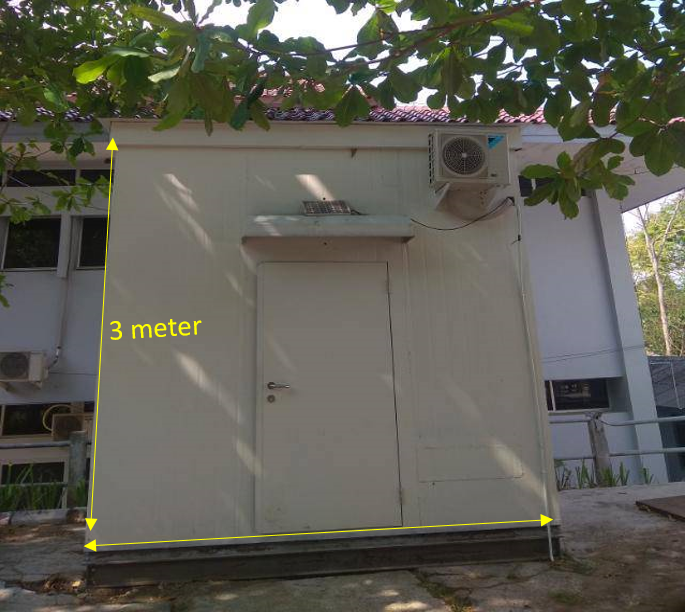
\includegraphics[width=0.45\textwidth]{figures/climatechamber}
	\caption{Foto \textit{Climate Chamber} DTNTF FT-UGM}
	\label{fig:1:fotochamber}
\end{figure}

\vspace{1mm}

\begin{figure}[!h]
	\centering
	\centering
	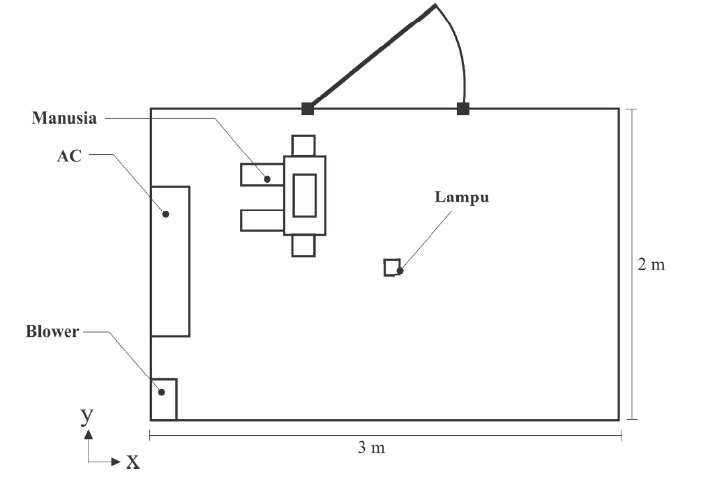
\includegraphics[width=0.65\textwidth]{figures/DenahChamber}
	\caption{Denah \textit{Climate Chamber} DTNTF FT-UGM\cite{skripsiIchfan}}
	\label{fig:1:denahchamber}
\end{figure}

\vspace{3em}

\textit{Climate chamber} merupakan suatu ruangan tertutup yang digunakan untuk menguji efek dari kondisi lingkungan yang ditentukan pada objek biologis, produk industri, bahan, dan/atau perangkat elektronik. Pada penulisan ini, \textit{climate chamber} yang dimaksud berfokus pada objek biologis mengenai penelitian kenyamanan termal. Dalam melakukan penelitian kenyamanan termal, peneliti tersebut membutuhkan suatu \textit{climate chamber} untuk dapat melakukan pengujian. Kondisi lingkungan termal di dalam \textit{climate chamber} dapat berubah sesuai dengan skema pengujian. Terdapat 6 faktor lingkungan termal yang mempengaruhi kenyamanan termal. Faktor lingkungan termal tersebut meliputi tingkat metabolisme tubuh, insulasi pakaian, suhu udara, suhu radian, kecepatan udara dan kelembapan \cite{ASHRAE55}.

\section{Perumusan Masalah}
\textit{Climate chamber} dapat terwujud jika kondisi iklim di dalamnya dapat dikendalikan sesuai dengan kebutuhan penelitian. Oleh karena itu, dibutuhkan suatu sistem kontrol yang mampu mengendalikan lingkungan termal pada \textit{climate chamber} dengan meninjau nilai \textit{steady-state error} suhu ruang dan kelembapan relatif. \textit{Climate chamber} memiliki banyak nilai masukan dan keluaran atau dikatakan sebagai sistem MIMO (\textit{multiple input multiple output}). Untuk dapat mengendalikan sistem MIMO, diperlukan sistem kontrol cerdas (\textit{intelligent control system}). Salah satu sistem kontrol cerdas yang dapat digunakan untuk sistem MIMO ini yaitu pengendali dengan menggunakan jaringan saraf tiruan (\textit{neural network controller}).

Perumusan masalah pada penelitian ini yaitu bagaimana merancang kontroler lingkungan termal berbasis jaringan saraf tiruan untuk dapat mencapai kondisi ajeg sesuai dengan skenario penggunaan \textit{climate chamber} DTNTF FT-UGM.

\section{Tujuan}
Penelitian ini bertujuan untuk membangun model kontroler berbasis jaringan saraf tiruan dengan meninjau nilai \textit{steady-state error} untuk mengendalikan lingkungan termal pada \textit{climate chamber} DTNTF FT-UGM.

\section{Batasan Masalah}
Berikut batasan masalah yang digunakan dalam penelitian ini:
\begin{enumerate}
	\item Data yang digunakan merupakan data simulasi IES-VE.
	\item Model \textit{plant} dibangun dengan menggunakan model jaringan saraf tiruan.
	\item Kinerja kontroler hanya ditinjau melalui nilai \textit{steady-state error} karena secara fisis respon transien termal pada bangunan berlangsung cukup lama.
	\item \textit{Climate chamber} dituntut untuk mampu menjaga kondisi lingkungan termal pada nilai tertentu dengan galat suhu kurang dari $\pm$1$^{\circ}$C dan galat kelembapan relatif kurang dari $\pm$10\%.
\end{enumerate}

\section{Manfaat}
Berikut manfaat dari penelitian ini:
\begin{enumerate}
	\item Penelitian ini diharapkan mampu mengembangkan ilmu pengetahuan dan aplikasinya di bidang fisika bangunan, sistem kontrol dan kecerdasan buatan.
	\item Penelitian ini diharapkan mampu menjadi referensi bagi praktisi kecerdasan buatan atau praktisi dalam pengembangan kenyamanan termal suatu bangunan.
	\item Penelitian ini diharapkan mampu memajukan perkembangan teknologi sistem bangunan di Indonesia.
\end{enumerate}
